% multiVector.net — slides for advisor presentation
% Compile with: latexmk -pdf slides.tex   (or pdflatex slides.tex twice)

\documentclass[aspectratio=169,11pt]{beamer}

\usepackage[utf8]{inputenc}
\usepackage[T1]{fontenc}
\usepackage{lmodern}
\usepackage{xcolor}
\usepackage{listings}
\usepackage{tikz}
\usepackage{amsmath, amssymb}
\usepackage{booktabs}

% ─── Theme ────────────────────────────────────────────────────────────────
\usetheme{metropolis}
\metroset{progressbar=frametitle, sectionpage=progressbar, numbering=fraction}

\definecolor{accent}{HTML}{1482C8}
\definecolor{accent2}{HTML}{0F9D57}
\definecolor{accent3}{HTML}{C30A3A}
\definecolor{ink}{HTML}{1E2433}
\definecolor{muted}{HTML}{8B93A4}
\definecolor{soft}{HTML}{F4F5F8}

\setbeamercolor{frametitle}{bg=ink, fg=white}
\setbeamercolor{progress bar}{fg=accent, bg=soft}
\setbeamercolor{normal text}{fg=ink}
\setbeamercolor{alerted text}{fg=accent3}

% ─── Code listings ────────────────────────────────────────────────────────
\lstdefinelanguage{gaexpr}{
  morekeywords={point, line, vector, color, exp, sqrt, sin, cos, abs, len, norm, inorm, triangle},
  morecomment=[l]{\#},
  sensitive=true,
}
\lstset{
  language=gaexpr,
  basicstyle=\ttfamily\small,
  keywordstyle=\color{accent}\bfseries,
  commentstyle=\color{muted}\itshape,
  numbers=none, frame=none,
  backgroundcolor=\color{soft},
  xleftmargin=4pt, framexleftmargin=4pt,
  framexrightmargin=4pt, framextopmargin=4pt, framexbottommargin=4pt,
  showstringspaces=false,
  literate=
    {>>>}{{\textcolor{accent}{>{>}>}}}3
    {->}{{$\rightarrow$}}2
    {<-}{{$\leftarrow$}}2
}

% ─── Metadata ─────────────────────────────────────────────────────────────
\title{\textbf{multiVector.net}}
\subtitle{A live, expression-driven \\ Geometric Algebra visualization environment}
\author{Étienne Harquin}
\institute{PhD candidate}
\date{\today}

% ─── Begin ────────────────────────────────────────────────────────────────
\begin{document}

\maketitle

% ── Section 1: Motivation ─────────────────────────────────────────────────
\section{Why this matters}

\begin{frame}{The GA tooling gap}
  Geometric Algebra is winning the theoretical battle in graphics, robotics
  and physics. But the tooling story has not kept pace.
  \begin{itemize}
    \item \alert{ganja.js} — powerful but bare; every demo is hand-rolled.
    \item \alert{GAlgebra / Clifford.jl} — symbolic, no live interaction.
    \item \alert{CGA viewer} — single algebra, fixed UI.
  \end{itemize}
  \vfill
  \textbf{No project today gives the user:}
  \begin{itemize}
    \item a uniform expression language across algebras,
    \item an interactive canvas where every object is draggable, and
    \item a clean way to define their own primitives.
  \end{itemize}
\end{frame}

\begin{frame}{The opportunity}
  GA needs a \textbf{Desmos-style standard} for visualizing multivector
  constructions — but mathematically faithful, algebra-pluggable, and
  open.

  \begin{center}
    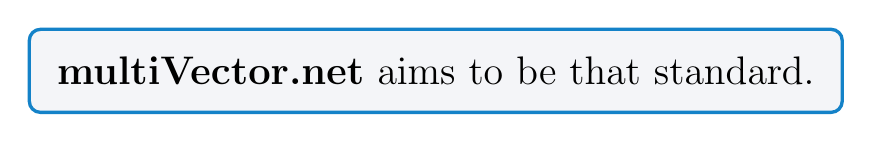
\begin{tikzpicture}
      \node[rounded corners, draw=accent, line width=1.2pt,
            inner sep=10pt, fill=soft]
        {\Large \textbf{multiVector.net} aims to be that standard.};
    \end{tikzpicture}
  \end{center}

  \begin{itemize}
    \item One language, many algebras.
    \item Expressions \emph{are} the construction — drag a point, every
          dependent object updates.
    \item User-extensible: define your own primitives in the language itself.
  \end{itemize}
\end{frame}

% ── Section 2: What it is ─────────────────────────────────────────────────
\section{What it is}

\begin{frame}{In one screenshot}
  \begin{columns}[T]
    \column{0.55\textwidth}
      A web application (React + Vite, SVG-rendered, \texttt{ganja.js}
      for GA primitives) where the entire construction lives in a
      left-hand expression panel.
      \begin{itemize}
        \item Type an expression \(\Rightarrow\) object appears.
        \item Drag the object \(\Rightarrow\) the expression updates.
        \item Edit the expression \(\Rightarrow\) the canvas redraws.
        \item Persistent: \texttt{localStorage} + named saved graphs.
      \end{itemize}

    \column{0.45\textwidth}
      \begin{center}
        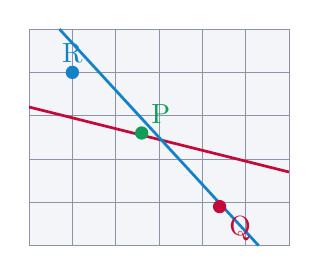
\begin{tikzpicture}[scale=0.55]
          \fill[soft] (-2,-2) rectangle (4,3);
          \draw[muted,very thin] (-2,-2) grid (4,3);
          \draw[accent3, line width=1pt] (-2,1.2) -- (4,-0.3);
          \draw[accent, line width=1pt] (-1.3,3) -- (3.3,-2);
          \filldraw[accent2] (0.6, 0.6) circle (4pt) node[above right]{P};
          \filldraw[accent3] (2.4,-1.1) circle (4pt) node[below right]{Q};
          \filldraw[accent]  (-1.0, 2.0) circle (4pt) node[above]{R};
        \end{tikzpicture}\\[4pt]
        \footnotesize Canvas (SVG, dark/light themed)
      \end{center}
  \end{columns}
\end{frame}

\begin{frame}[fragile]{The expression language}
  Every line is parsed, classified, evaluated, and rendered.
\begin{lstlisting}
P = point(1, 1)            # free draggable point
Q = point(2, 2)
L = P & Q                  # join: line through P and Q
M = exp(0.5 * e12)         # rotor (motor)
Q'= M >>> P                # sandwich transform
t = 0.5                    # animatable scalar slider
T = exp(t * (e01 + e02))   # translator parameterised by t
\end{lstlisting}
  \medskip
  Operators (tight $\to$ loose):
  \texttt{!} \texttt{\textasciitilde}\ $\succ$\
  \texttt{\textasciicircum} \texttt{\&} \texttt{|} \texttt{\S}\ $\succ$\
  \texttt{*} \texttt{/}\ $\succ$\
  \texttt{>{>}>}\ $\succ$\
  \texttt{+} \texttt{-}
\end{frame}

\begin{frame}{Type is a property of value, not syntax}
  Any expression is legal — its kind is determined by classifying the
  computed multivector:

  \begin{center}
  \begin{tabular}{ll}
    \toprule
    \textbf{kind} & \textbf{rendered as} \\
    \midrule
    finite point   & dot \\
    ideal point    & ring on horizon ellipse \\
    line           & infinite line \\
    ideal line     & dashed horizon ellipse \\
    vector         & arrow \\
    bivector       & oriented loop, area \(\propto \sqrt{|b|}\) \\
    rotor          & arc + angle label \\
    list           & polygon outline (if all points) \\
    \bottomrule
  \end{tabular}
  \end{center}

  \vfill
  Stroke widths and radii scale with the multivector's weight, so
  \texttt{5*e12} renders \emph{five times thicker} than \texttt{e12}.
\end{frame}

% ── Section 3: The architectural contribution ─────────────────────────────
\section{The architectural contribution}

\begin{frame}{Pluggable algebra adapters}
  Each algebra is a single file exposing one spec object:

  \begin{center}
  \begin{tabular}{ll}
    \toprule
    \textbf{spec field} & \textbf{role} \\
    \midrule
    \texttt{Algebra}, \texttt{arraySize} & ganja.js binding \\
    \texttt{bladeIndex}, \texttt{parseBladeName} & basis \& parser hook \\
    \texttt{classifyMV} & value \(\to\) kind \\
    \texttt{normalizeMVFinit/Ideal} & finite \& ideal norms \\
    \texttt{getRenderPlan} & value \(\to\) SVG primitive \\
    \texttt{supportedNodeTypes} & gates parser branches \\
    \texttt{INITIAL\_ITEMS} & showcase on load \\
    \bottomrule
  \end{tabular}
  \end{center}

  The parser, evaluator, expression engine and node-type registry are
  \alert{factory functions} bound to a spec — \textbf{adding a new GA is
  one new file}.

  \medskip
  \textbf{Already shipping:} PGA(2,0,1), VGA(2,0,0), R(0,1,0).
\end{frame}

\begin{frame}{Ganja delegation, single sign convention}
  Every GA primitive routes through ganja's built-in:

  \begin{center}
  \begin{tabular}{ll}
    \toprule
    \textbf{operation} & \textbf{routed to} \\
    \midrule
    dual \texttt{!A}            & \texttt{Algebra.Dual} \\
    reverse \texttt{\textasciitilde A} & \texttt{Algebra.Reverse} \\
    sandwich \texttt{M >>> A}   & \texttt{Algebra.sw} \\
    exponential \texttt{exp(V)} & \texttt{V.Exp()} (typed copy) \\
    \texttt{sqrt(motor)}        & log \(\to\) halve \(\to\) exp \\
    finite norm                 & \texttt{Algebra.Length} \\
    ideal norm                  & \texttt{Algebra.Length(Dual)} \\
    \bottomrule
  \end{tabular}
  \end{center}

  \medskip
  \textbf{No parallel implementations to drift.} Adding a new algebra
  inherits all of GA semantics for free — provided ganja supports it.
\end{frame}

% ── Section 4: Features ───────────────────────────────────────────────────
\section{Features (today)}

\begin{frame}[fragile]{Lists as first-class values}
\begin{lstlisting}
L = [P, Q, M >>> P, M*M >>> P]   # any types mix
~L                                # broadcast over list
M >>> L                           # transform every element
L1 ^ L2                           # elementwise wedge
len(L), L[i], L[i:j]              # length, index, slice
\end{lstlisting}
  All unary / binary operators broadcast or work elementwise.
  All-point lists draw a dashed polygon.
\end{frame}

\begin{frame}[fragile]{Smart norms, postfix accessors}
\begin{lstlisting}
|P & Q|              # smart norm (auto finite/ideal)
A.norm   A.inorm     # explicit finite / ideal norm
abs(s)               # scalar absolute value
A.e12                # blade coefficient extraction
A.e21                # permuted blades: A.e21 = -A.e12
\end{lstlisting}
  Plus norm / inorm toggle buttons per row that normalise the underlying
  value and propagate to dependents.
\end{frame}

\begin{frame}[fragile]{User-defined functions (just landed)}
\begin{lstlisting}
dist(A, B) = |A & B|         # function definition
midpoint(A, B) = (A + B) / 2
ln(A, B)   = A & B           # parameters are any object

d  = dist(P, Q)              # call anywhere
m  = midpoint(P, Q)
L  = ln(P, Q)
d2 = 2 * dist(P, Q) + 1      # nested in arithmetic
\end{lstlisting}
  Functions are values — captured globals propagate reactively,
  recursion is allowed with a depth cap, builtin-name collisions are
  rejected at parse time.
\end{frame}

\begin{frame}{Animation + interactivity}
  \begin{columns}[T]
    \column{0.5\textwidth}
      \textbf{Scalars are sliders}
      \begin{itemize}
        \item interval \texttt{(min, max, step)} per scalar,
        \item play \(\triangleright\) / pause; modes: pingpong, repeat,
              once, infinite,
        \item speed levels \(0.25\!\times\) to \(8\!\times\),
        \item any dependent object animates in lock-step.
      \end{itemize}

    \column{0.5\textwidth}
      \textbf{Direct manipulation}
      \begin{itemize}
        \item drag points, vector tail / tip independently,
        \item lock per item, hide per item,
        \item undo / redo (Ctrl-Z / Y), 100-step history with
              high-frequency drag coalescing,
        \item appearance per item: color, opacity, size, shape, label.
      \end{itemize}
  \end{columns}
\end{frame}

\begin{frame}{Polish that matters for adoption}
  \begin{itemize}
    \item \textbf{Light / dark theme} — every SVG color goes through CSS
          variables; theme switch cross-fades.
    \item \textbf{Adaptive grid} — major + minor (5-subdivision) gridlines,
          axis labels reposition when off-screen.
    \item \textbf{Persistence} — autosave to \texttt{localStorage} keyed
          per algebra; \texttt{Save} / \texttt{Open} named graphs.
    \item \textbf{Share} — encode the whole graph in a URL fragment for
          a one-click link.
    \item \textbf{Help modal} — full expression reference inline, no
          docs round-trip needed.
    \item \textbf{Error UX} — duplicate labels, invalid syntax, builtin
          collisions all surface as a red pastille + a single-line
          message; the row's value display is suppressed cleanly.
  \end{itemize}
\end{frame}

% ── Section 5: Why this matters for me ────────────────────────────────────
\section{Why this matters for the PhD}

\begin{frame}{A platform, not a demo}
  Most GA visualisation work is one-off: a fixed algebra, a fixed scene,
  a paper figure.

  \medskip
  \textbf{multiVector.net is general infrastructure.}
  \begin{itemize}
    \item Teaching: live derivations in a lecture, students fork the URL.
    \item Research: prototype a construction in minutes, save the JSON
          alongside the paper, drop a URL into reviewer correspondence.
    \item Community: a shared substrate where each algebra adapter and
          each saved graph compounds.
  \end{itemize}
\end{frame}

\begin{frame}{Concrete academic contributions}
  \begin{enumerate}
    \item \textbf{The algebra-adapter pattern.} A reproducible recipe
          for hosting any Clifford algebra in a single interactive UI.
    \item \textbf{The expression language.} A small but complete
          surface — binary GA operators, lists, smart norms, postfix
          accessors, label templates, user functions.
    \item \textbf{A reference implementation.} Open, web-native, no
          install — every figure in a future paper can be a live URL.
    \item \textbf{A library of saved constructions.} The JSON format is
          stable; each saved graph is a citable artefact.
  \end{enumerate}

  \medskip
  Each of these is a paper-sized contribution. Together they are the
  beginning of a community standard.
\end{frame}

\begin{frame}{Roadmap}
  \begin{itemize}
    \item More algebras: CGA, STA, 3D~PGA — each is one adapter file.
    \item Per-graph published URL \(\rightarrow\) versioned share links.
    \item Inline LaTeX rendering of expressions and labels.
    \item Replay of construction history as an animation
          (already have the undo / redo log — just expose it).
    \item Export: SVG, animated GIF, PDF figure with attached \texttt{.json}.
    \item A gallery: curated saved graphs as a discoverable corpus.
  \end{itemize}
\end{frame}

\begin{frame}{The ask}
  I would like to position the publication of
  \textbf{multiVector.net} —
  the system, the language, and the adapter pattern —
  as a contribution of my thesis.

  \medskip
  Short-term targets I can argue for:
  \begin{itemize}
    \item a tool paper (e.g.\ AGACSE, CGI tools track, or JOSS),
    \item a tutorial paper using the platform for derivations,
    \item a community-standard proposal (saved-graph JSON format).
  \end{itemize}

  \medskip
  \centering
  \alert{\textbf{Live demo:} \texttt{http://localhost:5174}}
\end{frame}

\begin{frame}[standout]
  Thank you, Vincent.\\[4pt]
  \footnotesize\normalfont
  Questions, sharpened criticism, and re-direction welcome.
\end{frame}

\end{document}
